\section{Utilities}


\begin{description}

\item[btkModifyImageUsingLookUpTable] This program modifies one image using a
look up table defined in a ascii file (2 columns, one for the original values,
one for the final values). Usage: \texttt{-i input\_image\_filename -t
input\_table\_filename -o output\_image\_filename}
  

\item[btkNrrdToNifti] This program convert an image from Nrrd file (*.nhdr
*.nrrd) to a Nifti file (*.nii). The conversion of a DWI image is possible by
using the option \texttt{-d}. Usage: \texttt{-i input\_nhdr\_header\_image -o
output\_nifti\_image}. Usage for DWI sequence: \texttt{-i
input\_nhdr\_header\_image -o output\_nifti\_image -v
gradient\_vectors\_filename -d}.

\item[btkNiftiToNrrd] This program convert a diffusion sequence in nifti
format\footnote{Currently there is no nifti standard for DWI, so DW images are
saved as a standard nifti sequence and two text files containing the b-values
(.bval) and the gradient directions (.bvec).} (*.nii, *.nii.gz) to the nrrd
format (*.nhdr). 

Usage: \texttt{-i input.nii -b bvalues.bval -g gradients.bvec -o output.nhdr
}

The list of optional parameters can be obtained by \texttt{btkNiftiToNrrd
--help}

  
  \item[btkReorientImageToStandard] Sometimes it is useful
to reorient the image to the standard orientation. This is necessary with fetal
images since in general the fetus is in a random orientation with respect to the
scanner.

Usage: \texttt{btkReorientImageToStandard -i image -o output -l landmarks}.
\texttt{landmarks} is a text file containing the spatial coordinates (in
RAS world coordinates) of points defining the left-right and the
posterior-anterior directions. This information must be organized as follows:

\begin{tabular}{cccc}
$l_x$ & $l_y$ & $l_z$ \\
$r_x$ & $r_y$ & $r_z$ \\
$p_x$ & $p_y$ & $p_z$ \\
$a_x$ & $a_y$ & $a_z$ 
\end{tabular}

where the points $l=(l_x, l_y, l_z)$ and $r=(r_x, r_y, r_z)$ define the
left $\rightarrow$ right direction, and the points $p=(p_x, p_y, p_z)$ and
$a=(a_x, a_y, a_z)$ define the posterior $\rightarrow$ anterior direction. Such
file can be easily generated by using Slicer\footnote{http://www.slicer.org}.

In order to create the landmarks by using Slicer you want to follow the
following procedure:

\begin{enumerate}
\item Open the high-resolution image by using the \textit{Volume} module.
\item Toogle on the visibility of all slices in the 3D view. This allows to
identify the left and right sides of the brain in the 2D views.
\item Place the landmarks $l$, $r$, $p$, and $a$ in this order by using
\texttt{[p]}.
\item Save the file (*.fcsv) by using the menu File $\rightarrow$ Save.
\item Edit the generated file by using any text editor to remove the additional
data about landmarks (i.e. the lines beginning with \texttt{\#} and text
'around' the coordinates).
\end{enumerate}


\begin{figure}[t]
\centering
\begin{tabular}{ccc}
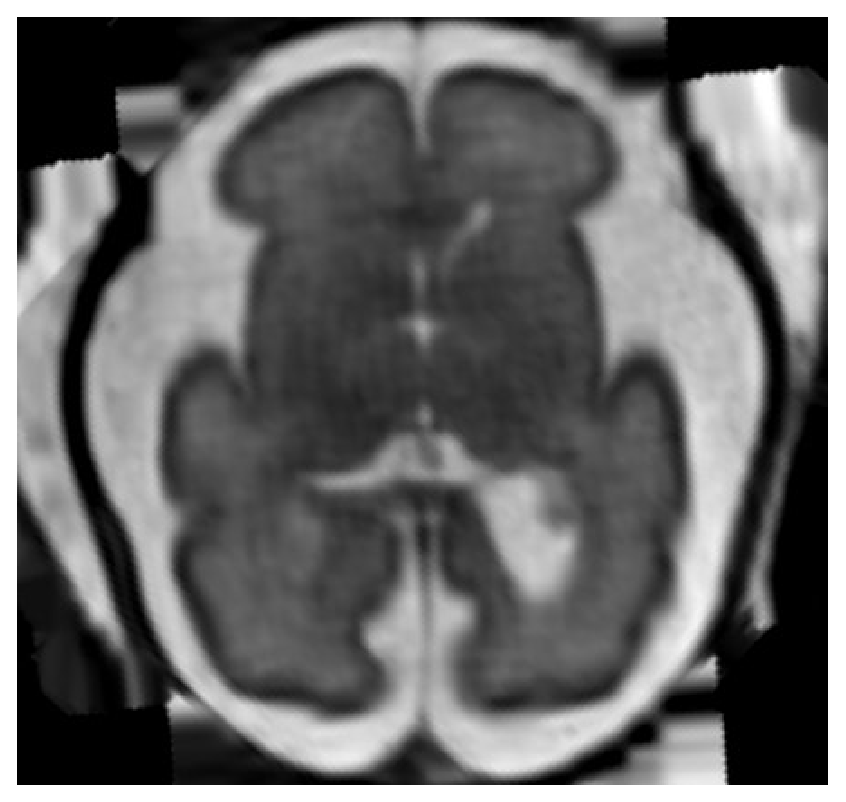
\includegraphics[width=0.3\columnwidth]{hr_axl.eps}&
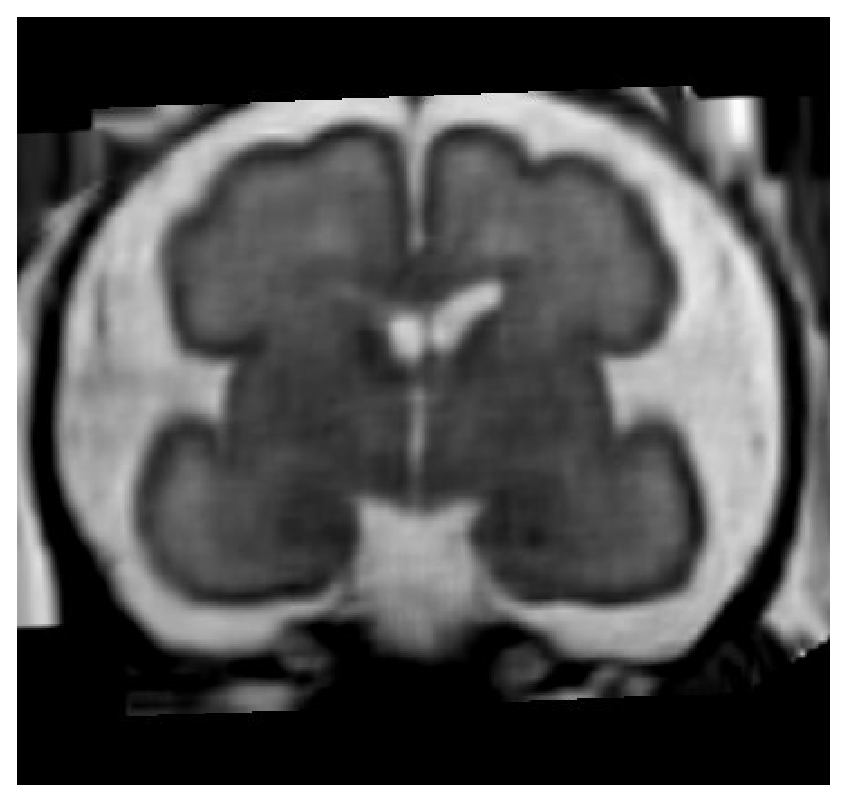
\includegraphics[width=0.3\columnwidth]{hr_cor.eps}&
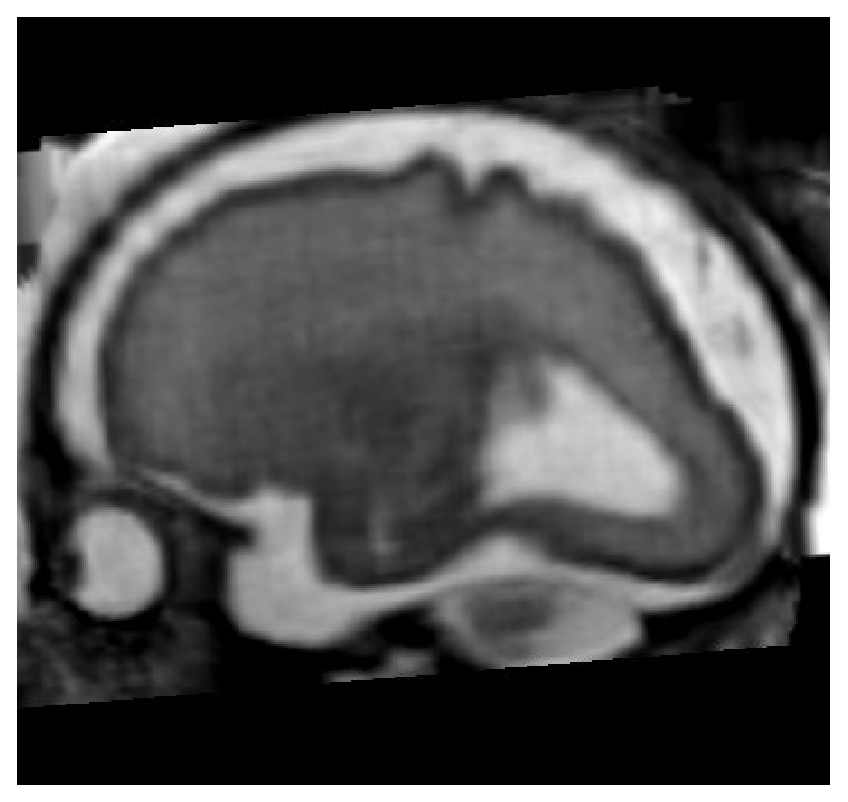
\includegraphics[width=0.3\columnwidth]{hr_sag.eps}\\
{(a)}&{(b)}&{(c)}\\
\end{tabular}
\caption{Example of an anatomical reconstruction of a fetal brain by using
\texttt{btkImageReconstruction}. (a) axial, (b) coronal, and (c) sagital view.}
\label{fig:reconstruction}
\end{figure}

\begin{figure}[t]
\centering
\begin{tabular}{cc}
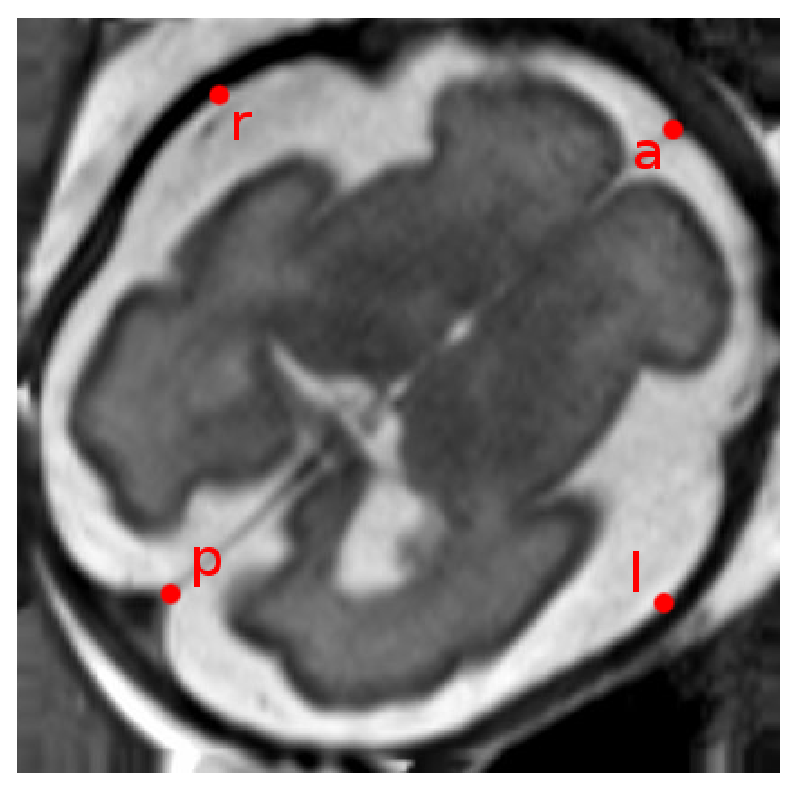
\includegraphics[width=0.35\columnwidth]{lmks_axial.eps}&
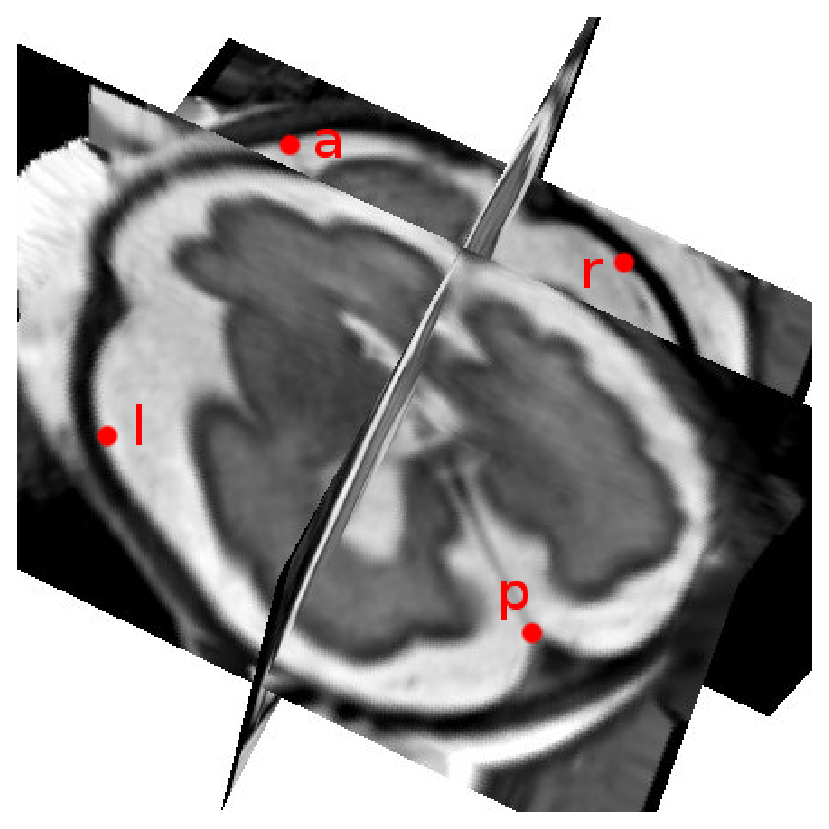
\includegraphics[width=0.35\columnwidth]{lmks_3D.eps}\\
{(a)}&{(b)}\\
\end{tabular}
\caption{Placement of landmarks by using Slicer. (a) axial slice, (b) 3D view.}
\label{fig:landmarks}
\end{figure}

  \item[btkReorientDiffusionSequenceToStandard] Reorients a DW sequence
to the standard orientation. This is necessary with fetal images since the fetus
is in a random orientation with respect to the scanner. This is particularly
important in DWI because colormaps lack of significance, which makes difficult
the identification of specific bundles 

Usage: \texttt{btkReorientDiffusionSequenceToStandard -i image -g
gradients.bvec -l landmarks -o output -c gradients\_corr.bvec}.

\texttt{landmarks} is a landmarks file obtained as explained above.
\texttt{gradients\_corr.bvec} is a text file containing the corrected
gradient table.
\end{description}
